\documentclass[
  11pt,
  fleqn
]{article}
% [fleqn] left-aligns all equations

% fonts

\usepackage[T1]{fontenc} % Apparently this
% https://tex.stackexchange.com/questions/287312/font-not-loadable-metric-data-not-found-or-bad
\usepackage[full]{textcomp}
\usepackage[final,expansion=alltext,nopatch=footnote]{microtype}
\usepackage{csquotes} % suppress warning from `babel`
\usepackage[english]{babel}
\usepackage[fleqn]{mathtools}
\usepackage[cal=boondoxo]{mathalpha} % mathcal

\usepackage{amsthm} % gives proof environment:
% https://www.overleaf.com/learn/latex/Theorems_and_proofs

\usepackage{newtxtext}
% \usepackage{txfonts} % See
% https://tex.stackexchange.com/questions/444243/symbols-not-showing-up

% These need to be after newtxtext
\usepackage[varqu,varl]{inconsolata} % sans serif typewriter
% \usepackage{cabin} % sans serif - ugly

\usepackage[bigdelims,vvarbb]{newtxmath} % bb from STIX % "should be
% loaded AFTER the text font" -
% https://mirrors.mit.edu/CTAN/fonts/newtx/doc/newtxdoc.pdf

% geometry of the page

\usepackage[
  % top=1in,
  % bottom=1in,
  % left=1in,
  % right=1in
]{geometry}

% paragraph spacing

\setlength{\parindent}{0pt}
\setlength{\parskip}{1.5ex plus 0.4ex minus 0.2ex}

% useful packages

% \usepackage{natbib} % incompatible with BibLaTeX
\usepackage{epsfig}
\usepackage{url}
\usepackage{bm}
\usepackage{blindtext}

% Leon additions

\usepackage{enumitem} % allows for enumerate[resume]

\usepackage{booktabs}

\usepackage[
  style=authoryear-comp,
  natbib=true,
  % refsection=chapter,
  url=false,
  doi=true,
  isbn=false,
  date=year %
  % https://tex.stackexchange.com/questions/55780/disable-month-in-biblatex-bibliography
]{biblatex} % natbib=true allows \citep
% Clear "visited on"
% https://tex.stackexchange.com/questions/400384/how-to-disable-biblatex-showing-visited-on-on-the-references
\AtEveryBibitem{
  \clearfield{urlyear}
  \clearfield{urlmonth}
  \clearfield{eprint} % remove PMID %
  % https://tex.stackexchange.com/questions/250784/removing-eprint-and-eprinttype-in-citation-notes
}

\usepackage{graphicx}
% ensures figures stay in their section
% https://tex.stackexchange.com/questions/279/how-do-i-ensure-that-figures-appear-in-the-section-theyre-associated-with
\usepackage[section]{placeins}

% Section formatting using titlesec
\usepackage{titlesec}
\titleformat*{\section}{\singlespacing\sffamily\Large}
\titleformat*{\subsection}{\singlespacing\sffamily\large}
% \titleformat*{\subsubsection}{\itshape}
\titleformat*{\paragraph}{\itshape}
\titleformat{\chapter}{\singlespacing\sffamily\Huge}{{\thechapter}}{1em}{}

% center figures by default
\makeatletter
\g@addto@macro\@floatboxreset\centering
\makeatother
% italic figure captions
\usepackage[format=plain,
  textfont=it,
]{caption}

% simple TO DO and comment macros
\usepackage[
  % https://tex.stackexchange.com/questions/4503/how-do-i-specify-color-in-rgb-using-hypersetup-in-hyperref
  dvipsnames,svgnames,x11names
]{xcolor}
\newcommand\todo[1]{\textcolor{orange}{[#1]}}% simple TO DO macro
\newcommand\comment[1]{\textcolor{red}{[#1]}}

\usepackage{url}
\usepackage[
  hidelinks,
  pdfa % Required for valid pdf/a output:
  % https://tex.stackexchange.com/questions/431022/pdf-a-validation-problem-the-f-key-is-missing
]{hyperref}
\hypersetup{
  % colorlinks,
  % linkcolor=RoyalBlue4,
  % citecolor=PaleVioletRed4,
  % urlcolor=Firebrick4
}

\newcommand{\indsim}{\overset{\mathrm{ind}}{\sim}}
% https://tex.stackexchange.com/questions/60545/should-i-mathrm-the-d-in-my-integrals
\newcommand*\diff{\mathop{}\!\mathrm{d}}
\newcommand*\Diff[1]{\mathop{}\!\mathrm{d^#1}}
\newcommand{\e}{\mathrm{e}}
\newcommand{\E}{\mathrm{E}}
\renewcommand{\P}{\mathrm{P}}
\newcommand{\N}{\mathrm{N}}
\newcommand{\diag}{\mathrm{diag}}
\newcommand{\ave}{\mathrm{ave}}
\newcommand{\Var}{\mathrm{Var}}
\newcommand{\Cov}{\mathrm{Cov}}
\newcommand{\cov}{\mathrm{cov}}
\newcommand{\sd}{\mathrm{sd}}
\newcommand{\var}{\mathrm{var}}
\newcommand{\corr}{\mathrm{corr}}
\renewcommand\vec{\boldsymbol}

% Overlap-specific
\newcommand{\rank}{R}
\newcommand{\rmax}{m}
\newcommand{\rgap}{r^\text{gap}}
\newcommand{\Ngap}{N_1^\text{gap}}
\newcommand{\pigap}{\pi_1^\text{gap}}

% For appearance of block matrices
% https://tex.stackexchange.com/questions/495903/horizontal-and-vertical-lines-in-pmatrix
\renewcommand{\arraystretch}{1.5}

% Theorem-type environments
\newtheorem{definition}{Definition}[section]
\newtheorem{result}[definition]{Result}
\newtheorem{claim}[definition]{Claim}

% From Datta template
% https://github.com/bibekanandadatta/JHU-Dissertation-Template

\usepackage{setspace}                         % sets space between lines

%%%% JH Library requirement (DO NOT CHANGE)
\def\GlobalMargin{1.0in}                      % margin on all sides
% \def\PrintingOffset{0.5in}                  % additional left
% margin for the printed copy
\def\PrintingOffset{0.0in}
\def\MainTextSpacing{\singlespacing}        % double-spaced main text
% \def\MainTextSpacing{}
\def\CaptionStretch{1.1}                    % to match 2x spacing
% \def\CaptionStretch{1.0}

\captionsetup{font={stretch=\CaptionStretch}}

\geometry{
  letterpaper,
  margin=\GlobalMargin,
  bindingoffset=\PrintingOffset,
  nomarginpar,
  % includehead,
  % headheight=\HeaderHeight,
  % headsep=\HeaderSpace,
  includefoot,
  heightrounded
}

%%%% BIBLIOGRAPHY ITEMS
\def\BibTextSpacing{\onehalfspacing}         % single-spaced bibliography
% \def\BibTextSpacing{\singlespacing}         % single-spaced bibliography
\def\BibItemSpacing{\baselineskip}          % spacing between
% bibliographic items in reference

%%%% UNNUMBERED CHAPTERS, SECTION, and SUBSECTION COMMAND for ADDING to TOC
%% removes the 'Chapter #' title while keeping it listed in the TOC
\newcommand\chap[1]{%
  \chapter*{#1}%
  \markboth{#1}{}
\addcontentsline{toc}{chapter}{#1}}

%% removes the 'Section #' title while keeping it listed in the TOC
\newcommand\sect[1]{%
  \phantomsection
  \section*{#1}%
\addcontentsline{toc}{section}{#1}}

%% removes the 'Subsection #' title while keeping it listed in the TOC
\newcommand\subsect[1]{%
  \phantomsection
  \subsection*{#1}%
\addcontentsline{toc}{subsection}{#1}}

%% removes the 'Subsubsection #' title while keeping it listed in the TOC
\newcommand\subsubsect[1]{%
  \phantomsection
  \subsubsection*{#1}%
\addcontentsline{toc}{subsubsection}{#1}}

% Correct matrix for double spacing
% https://tex.stackexchange.com/questions/137004/matrix-within-equation/137009#137009
\makeatletter
\def\env@matrix{\hskip -\arraycolsep
  \let\@ifnextchar\new@ifnextchar
  \linespread{1}\selectfont
  \renewcommand{\arraystretch}{1.2}%
\array{*\c@MaxMatrixCols c}}
\makeatother

% Footnotes must be 2 points less than main text but larger than 8pt
\usepackage{footmisc}
\renewcommand{\footnotesize}{\fontsize{9pt}{11pt}\selectfont}

% For including CV
\usepackage{pdfpages}

% Generate PDF/A (archival format)
% https://webpages.tuni.fi/latex/pdfa-guide.pdf
\usepackage[a-1b,mathxmp]{pdfx}

\usepackage[
  nottoc % Don't include TOC in TOC
]{tocbibind}

% Redefine `abstract`s so they can be at the start of each chapter
% don't cause the page numbering to reset
% https://tex.stackexchange.com/a/4857
\newenvironment{myAbstract}{
  \rightskip.5in
  \leftskip.5in
  % \itshape
}{}

% For writing/planning purposes: show paragraph level in TOC
\setcounter{secnumdepth}{2}

\addbibresource{bibliography.bib}
\graphicspath{{fig/}}

\title{Notes on Ordinal Measures of Association and Effect}
\author{Leon Di Stefano}
\date{\today}

\begin{document}

% \maketitle
\section*{Notes on Ordinal Measures of Association and Effect}
Leon Di Stefano

\section{Some definitions}

A good reference is \citet{kruskalOrdinalMeasuresAssociation1958}.

Two high level definitions/distinctions:

\begin{itemize}

  \item \textbf{``measures of association''
    versus ``measures of effect''}
    I want to distinguish measures of association, which measure the
    extent to which $p(x, y)
    \neq p(x)p(y)$, from ``measures of regression'' or ``measures of
    effect'' which measure differences among the conditional
    distributions $p(y \mid x)$ as $x$ varies, i.e.
    characterize the function $x \rightarrow p(y \mid x)$ (and in the
      simplest case when $x$ is binary, are comparisons of $p(y \mid
    x=1)$ to $p(y \mid x=0)$, as in treatment effects).

    How to assess whether a given measure is about ``association''
    versus ``effect''?

    In the strongest, fully nonparametric sense -- that is, without
    considering specific measures of effect or association -- ``absence of
    association'' and ``absence of effect'' coincide. But that
    doesn't help in characterizing what should count as a measure of
    association versus a measure of effect.

    Here are some ways to potentially formalize the difference:

    \begin{itemize}

      \item One way is to require that the formula for a measure
        of association should be symmetric in $x$ and $y$, whereas a
        measure of effect may not (or should not) be.

      \item Another way might be to require that measures of effect should be
        invariant to changing the marginal distribution of $x$ while leaving the
        conditionals intact (for example reweighting the joint
          distribution using
        weights that are a function only of $x$).

    \end{itemize}
    The second definition may be overly restrictive.

    Note that the odds ratio for a $2\times 2$ table satisfies both
    definitions above! It is a function of only the conditional
    distributions, but is also symmetric.

  \item \textbf{What does it mean to say that a measure is
    ``ordinal''?} Some measures of association or effect
    depend only on the probabilities attached to $x$ and
    $y$ values and not on any structure or properties of the $x$ and
    $y$ variables themselves. Call them ``distribution-only'' measures.

    An example is the mutual information for discrete $x, y$ given by
    \[ \sum_{x,
      y} p(x, y) \log\left(\frac{p(x, y)}{p(x) p(y)}\right) = \ave \left[
    \log\left(\frac{p(x, y)}{p(x) p(y)}\right) \right]. \]

    Others depend on the joint distribution of $x$ and $y$, but also
    only properties of $x$ and $y$ values themselves. Call these
    ``variable-involving'' measures.

    Covariance, for example, given by
    \[\cov(x, y) = \ave (x - \overline{x})(y - \overline{y}),\] is
    not like this,
    which depends on being able to add, subtract, scale, and
    multiply the associated variables.

    The importance of this definition is that when we consider
    ordinal measures of association and effect, we mean measures that
    are \emph{variable-involving, but through ordinal properties of
    the variables only}.

\end{itemize}

I'm not sure if there are more correct names for these in the literature.

\paragraph{Purely ordinal measures of association and effect} Ordinal measures
of effect should be functions of $y$ values but only through their ordering,
and ordinal measures of association should be functions of $x$ and
$y$ values, but only through their respective orderings. This means
they can make use of
\begin{itemize}
  \item Relations like $=, \leq, \geq$, which are functions of
    \emph{pairs} of values of a variable
  \item Quantiles (e.g. median) and order statistics, which are
    aspects of \emph{distribution} of an ordinal variable that depend
    only on the ordering; e.g. \[\text{median} = \text{solve}_q \left\{\Pr(x
    \leq q) = 0.5\right\}. \]
  \item Replacing $x$ and $y$ values by their ranks, or by the
    associated ``ridit'' (which is a rescaling of the ``midrank'',
    \citet{agrestiAnalysisOrdinalCategorical2010}) or eCDF
\end{itemize}

Another way of putting this
is that the measures should be
invariant under strictly monotone transformations of $x$ and $y$
\citep{kruskalOrdinalMeasuresAssociation1958}. However, this seems to
presume that the ordinal variables come from underlying numeric
variables, which may not be the case.

\paragraph{A 2$\times$2 breakdown} I think we have the options
\begin{itemize}
  \item $x$ ordinal, $y$ ordinal, measure of effect
  \item $x$ ordinal, $y$ ordinal, measure of association
  \item $x$ binary, $y$ ordinal, measure of effect
  \item $x$ binary, $y$ ordinal, measure of association
    (\textbf{requirement of symmetry means this is probably subsumed
    in the ordinal/ordinal case})
\end{itemize}
... which generalize the measures of effect and measures of
association for 2x2 tables.

\section{Constructing measures of association and effect using
independent draws}

The operators $=, <, >$ are
functions of \emph{pairs} of values. I think this is
one way to motivate the
following ``devices'' which can be used to construct ordinal measures of
association and
effect:
\begin{itemize}
  \item For measures of association, consider drawing
    \textbf{independent pairs} $z_1 = (x_1, y_1)$ and $z_2 = (x_2, y_2)$
    from $p(x, y)$.

    Then when $x$ and $y$ are ordinal, we can use $<, =, >$ to
    construct the disjoint events
    concordance $C(z_1, z_2)$, discordance $D(z_1, z_2)$, and ties
    in one or both
    variables $T_x(z_1, z_2), T_y(z_1, z_2), T_{xy}(z_1, z_2)$.

    We get measures of association by understanding the probabilities
    of these events under independence.

    Specifically,
    \begin{itemize}
      \item $\Pr(C) = \Pr(D)$ [I think]
      \item $\Pr(T_{xy}) = [\Pr(T_x) + \Pr(T_{xy})]\times [\Pr(T_y) +
        \Pr(T_{xy})]$
      \item The probabilities of $C, D, T_x, T_y, T_{xy}$ (5
          probabilities, 4 degrees
        of freedom) can be
        parametrized by only $T_x$, $T_y$. [I think]
    \end{itemize}

  \item For measures of effect when $x$ is binary, considering drawing
    \textbf{independent values of the response} $y_0
    \sim p(y \mid x = 0)$ and $y_1 \sim p(y \mid x = 1)$.

    Then when $y$ is ordinal we can consider the events $G = y_1 >
    y_0$ (``greater than''), $L = y_1 < y_0$ (``less than''), $E =
    y_1 == y_0$ (``equal to'').

    We get measures of effect by understanding the probabilities of these events
    under equality of distributions, or equivalently under
    independence of $y$ and binary $x$. Specifically, when the
    distributions are the same $\Pr(G) + \Pr(E)/2 = 1/2$
    and $\Pr(G) = \Pr(L)$.

\end{itemize}

\paragraph{Connection between the two devices}What's the connection
between the ``independent pairs'' and ``independent response values''
devices above? Consider $y$ ordinal
and $x$ \emph{dichotomous ordinal} with $x = 0, 1$ and $0 < 1$. (This
seems always true when we're considering an effect measure.) Then
\begin{itemize}
  \item The second sampling scheme is like the first but conditional
    on $x_1 \neq x_2$ [... I think].
  \item $C = G$ and $D = L$, and $T_y = E$. The events $T_x$ and
    $T_{xy}$ are excluded by construction.
\end{itemize}
That is, \textbf{every ordinal measure of association should
specialize to an ordinal measure of effect when $x$ is binary}
(though as discussed above \emph{maybe} we want this to be a true measure of
effect that \textbf{doesn't depend on the $x$-probabilities}).

Two asides:

\begin{itemize}
  \item \citet{kruskalOrdinalMeasuresAssociation1958} even
    considers further involving \emph{three} independent copies of
    the variables.
  \item Covariances and least squares regression coefficients can also be
    expressed using the ``pairs of draws'' device:\footnote{ I believe this is
      connected with
      $U$-statistics.\url{https://stats.stackexchange.com/questions/612496/linear-regression-vs-average-of-slopes}
      See also \url{https://www.fharrell.com/post/po/} discussion of
      Mann-Whitney. This also says that \textbf{it's possible to
        convert between Wilcoxon statistic, Somers' $D$, concordance
      probability, \emph{and} the Spearman rank correlation.}
    } \[ \cov(x, y) = \frac{1}{2}\ave(x - x')(y - y') \\ b_{yx} =
      \frac{\ave (y -
      y')(x - x')}{\ave (x - x')^2} = {\ave \left(w \times
      \text{pair-slopes}\right)}
    \]
    ... where the weight $w_{ij}$ is ${\Delta x^2}\big/{\sum \Delta x^2}$.

    As covered below some of the measures can be interpreted in terms
    of means and (co)variances and regression coefficients.
\end{itemize}

\paragraph{How this works in finite samples} When we have a dataset with $N$
values of $(x, y)$, then there are $N(N-1)$ \emph{ordered} pairs. If $x$ is
dichotomous with $n_0$ values of 0 and $n_1$ values of 1, \todo{...continue
this logic}.

\paragraph{Expression as regressions} Sometimes it's useful to
re-express these measures in terms of expectations, covariances,
correlations, etc. of e.g. ranks, or signs of differences in ranks, or

\begin{itemize}
  \item Spearman's $\rho$ = correlation of ranks
  \item Correlation of normal scores of ranks
\end{itemize}

\section{Graphical interpretations}

ROC curve: plots sensitivity against (1 - specificity). (Unscaled:
true positives against false positives.) That is, $\Pr(\text{correct}
\mid t, \text{False})$ against $\Pr(\text{incorrect} \mid t, \text{False})$..

P-P plot: plots eCDF(y) against eCDF(x) (or CDF($x$) in the case of a
theoretical reference distribution). Note that $x$ and $y$ are
ordinal but do not necessarily share the same space.

I think that \textbf{choosing a point at random in $PP$-space
  corresponds to independently choosing $x$ and a $y$ from their
marginal distributions}. Yes: see Figures
\ref{fig:pp_effect_measures} and \ref{fig:pp_ridit}.

What's the connection? Let $y$ be the score associated with the
diagnostic test and assume that a smaller $y$ is associated with a
decision in favor of $X =$ True.

Then the ROC curve is a plot of $\Pr(Y \leq t \mid X = \text{True})$
(which is just sensitivity)
versus $\Pr(Y \leq t \mid X = \text{False})$ (which is just 1 -
specificity) -- that is, a plot of cdf($y \mid x = 1$) versus cdf($y
\mid x = 0$)

\begin{figure}
  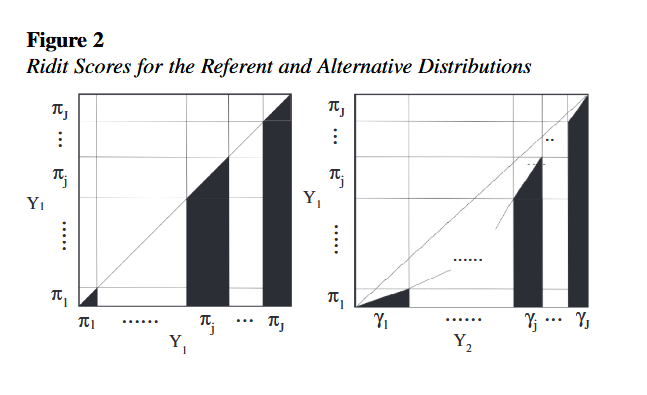
\includegraphics[width=5in]{PP_or_ridit_interpretation_of_AUROC.png}
  \caption{PP-plot/ridit interpretation of AUROC, from
  \citet{smithsonReceiverOperatingCharacteristic2023}}
  \label{fig:pp_ridit}
\end{figure}

\begin{figure}
  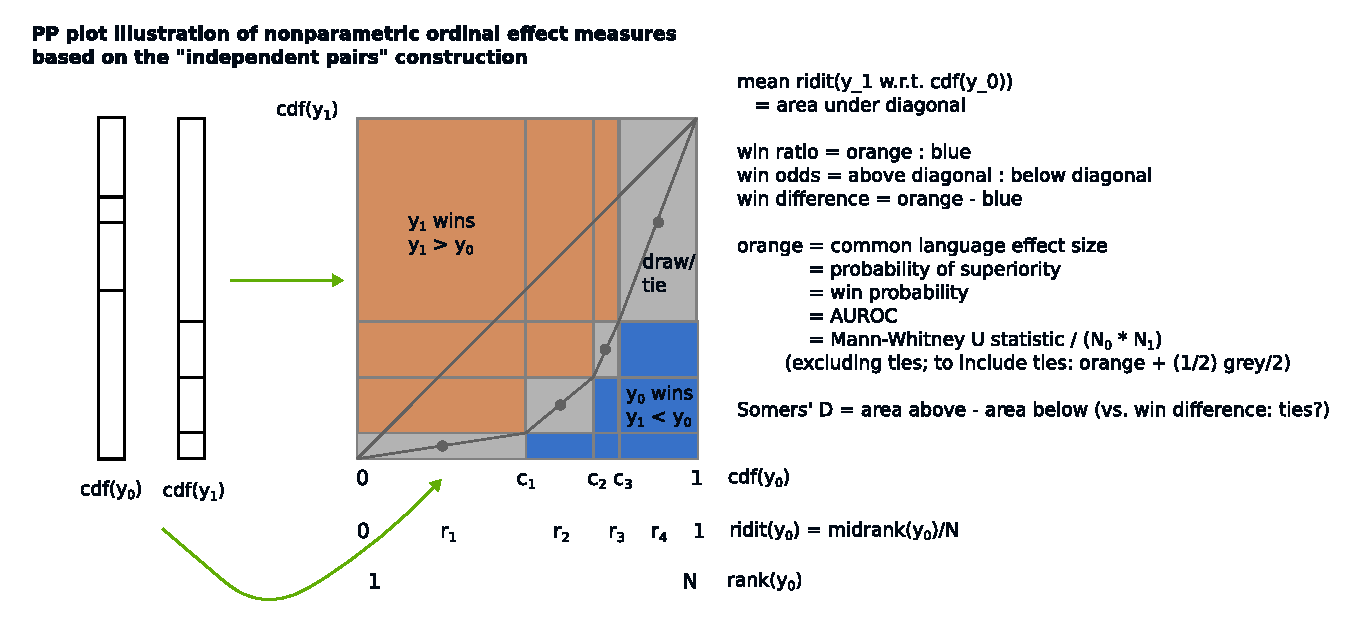
\includegraphics[width=6.5in]{effect_measures_pp_plot.pdf}
  \caption{PP-plot/ridit interpretation of other effect measures,
  based on Figure \ref{fig:pp_ridit}}
  \label{fig:pp_effect_measures}
\end{figure}

\begin{figure}
  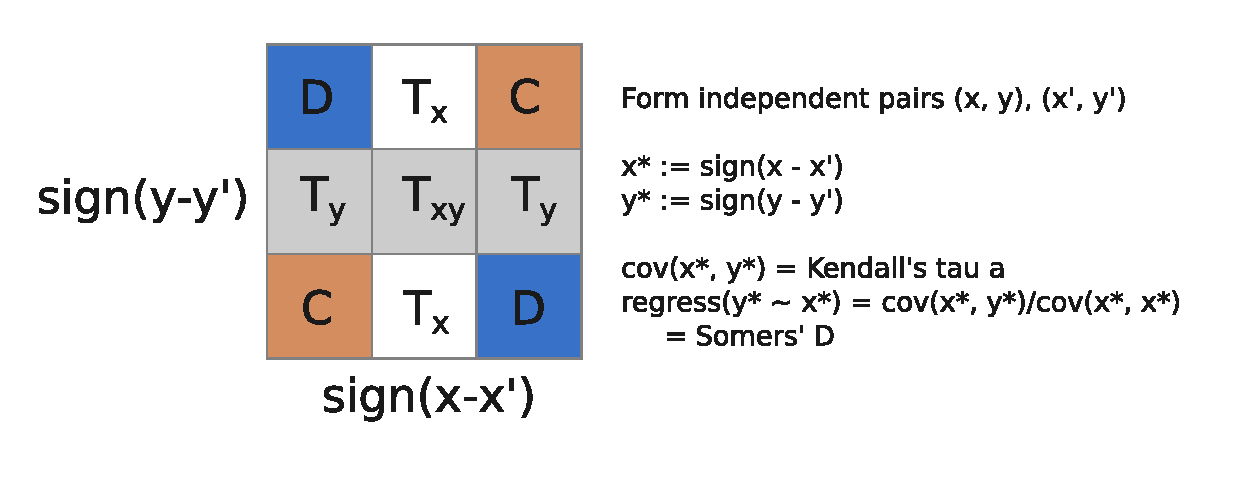
\includegraphics[width=6.5in]{ordinal_xy_pair_signs_plot.pdf}
  \caption{Plot illustrating components of ordinal-ordinal measures
    of association and effect. Regions of the same color in this plot
    and in the PP plot Figure \ref{fig:pp_effect_measures} correspond
    when $x$ is binary. Note that $x^*$ and $y^*$ have symmetric
  distributions centered at 0 by construction.}
  \label{fig:ordinal_xy}
\end{figure}

\section{List of measures of association and effect}

\subsection{Measures of effect}

\subsubsection{Binary \emph{x}, ordinal \emph{y}}

\begin{itemize}
  \item \textbf{Mann-Whitney $U$ statistic and its limit} Rescaling
    gives estimate of ``common language effect size'' = probabilistic
    index = probability of superiority = AUROC = win probability.... See
    \url{https://en.wikipedia.org/wiki/Mann%E2%80%93Whitney_U_test#Common_language_effect_size}.
      Note that this page also mentions a statistic ``$\rho$''
      which is the version incorporating ties, i.e.~$\Pr(Y > X) +
      0.5 \times \Pr(Y = X)$.
      % \item \textbf{Wilcoxon statistic and its limit} Signed rank
      % test. Either a
      %   single sample (in which case testing "whether the data come from
      %   a symmetric distribution with a specified center") or paired samples.
    \item \textbf{Win probability} Measure of effect. In terms of
      Somers' D it's
      $\frac{\text{SD} + 1}{2}$
    \item \textbf{Win difference} Seems to be the specialization of
      Kendall's Tau (see below).
    \item \textbf{Win ratio} Pr(win)/Pr(loss) (either matched or unmatched)
    \item \textbf{Win odds} Differs from the win ratio by incorporating ties
    \item \textbf{Mean ridit}
  \end{itemize}

  \subsubsection{Ordinal \emph{x}, ordinal \emph{y}}

  \begin{itemize}
    \item \textbf{Somers' $D$} \citep{newsonInterpretationSomersFour,
      newsonParametersNonparametricStatistics2002} Somers $D$ $=$ win
      difference (when $X$ is binary) = risk difference (when $X$ and
      $Y$ are binary)
    \item \textbf{Harrell's $C$ index} Equal to ROC with a binary outcome. A
      transform of Somers' $D$
    \item \text{Concordance/discordance ratio} = analogue of win
      ratio for ordinal-ordinal association
      \citet{newsonParametersNonparametricStatistics2002}. Reduces to
      odds ratio when $x$ and $y$ are binary.
  \end{itemize}

  Are there others in \citet{agrestiAnalysisOrdinalCategorical2010}
  that I'm missing?

  \subsection{Measures of association}

  \subsubsection{Ordinal \emph{x}, ordinal \emph{y}}

  \begin{itemize}
    \item \textbf{Kendall's $\tau$ ($a$ and $b$ and $c$ forms --
      \textbf{distinguish these})}
      From \citet{newsonParametersNonparametricStatistics2002}
      \begin{align*}
        \tau_a(X,Y)
        &= \mathrm{E}\left(\text{sign}(X_1-X_2)\text{sign}(Y_1-Y_2)\right) \\
        &=
        \mathrm{Cov}(\left(\text{sign}(X_1-X_2)\text{sign}(Y_1-Y_2)\right)) \\
        &= \Pr\left(\text{concordant}\right) -
        \Pr\left(\text{discordant}\right) = \Pr\left(C\right) -
        \Pr\left(D\right)
      \end{align*}
      Note that ``$x_1 - x_2$'' has no meaning for ordinal variables, but
      sign$(x_1 - x_2)$ is a meaningful abuse of notation.

      Somers' $D = D_{yx}$ is the associated regression coefficient
      $\tau_a(X, Y)/\tau_a(X, X)$

      Kendall's $\tau_b$ is the associated \emph{correlation} coefficient
      and is given by
      \[
        \tau_b = \text{sign}(\tau_a) \times \sqrt{D_{yx} D_{xy}}
      \]

    \item \textbf{Goodman-Kruskal $\gamma$} \[\gamma :=\frac{\Pr(C) -
      \Pr(D)}{\Pr(C) + \Pr(D)}\] Wikipedia: specializes to Yule's $Q$
      for 2x2 tables.

  \end{itemize}

  \newpage

  \section{References}
  \printbibliography

  \end{document}